\chapter{Prototype}
\section{RPi2 Hardware}
\pageauthor{Paul Zwölfer}
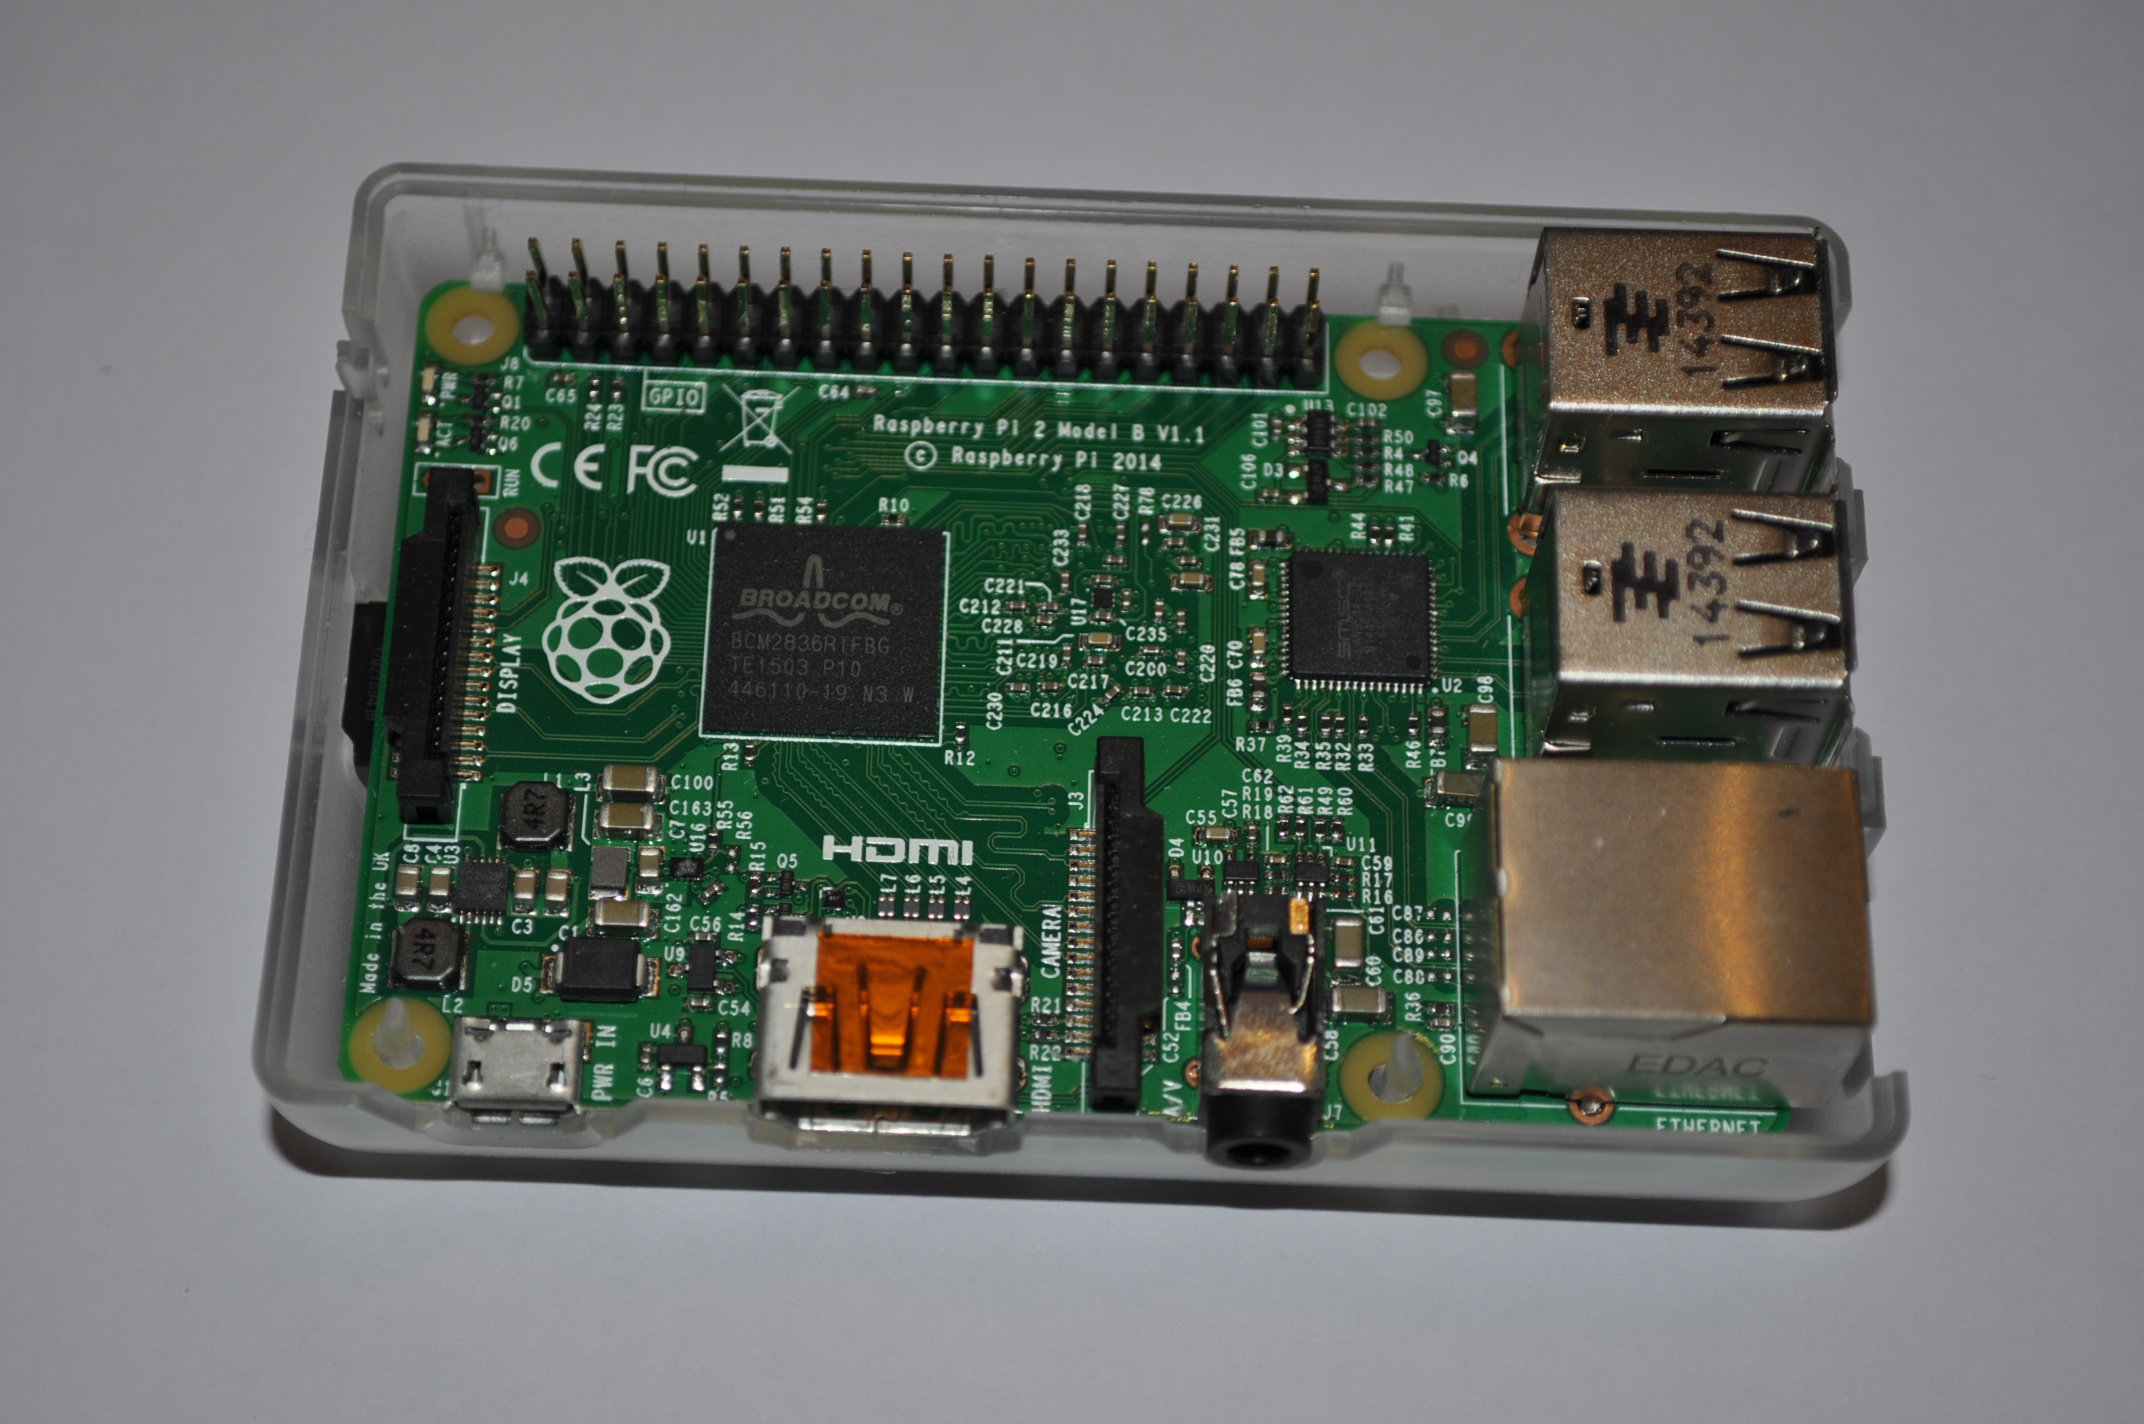
\includegraphics[width=0.48\textwidth]{bilder/DSC_0429}
\subsection{GPS Module}
The \gls{gps} module had to be soldered to the \gls{gpio} pins. We didn't trust our soldering skills and tried to avoid damage to the module. But it turned out that we needed a maximum of reliability for the connection and decided to solder the plug to the circuit board.\newline
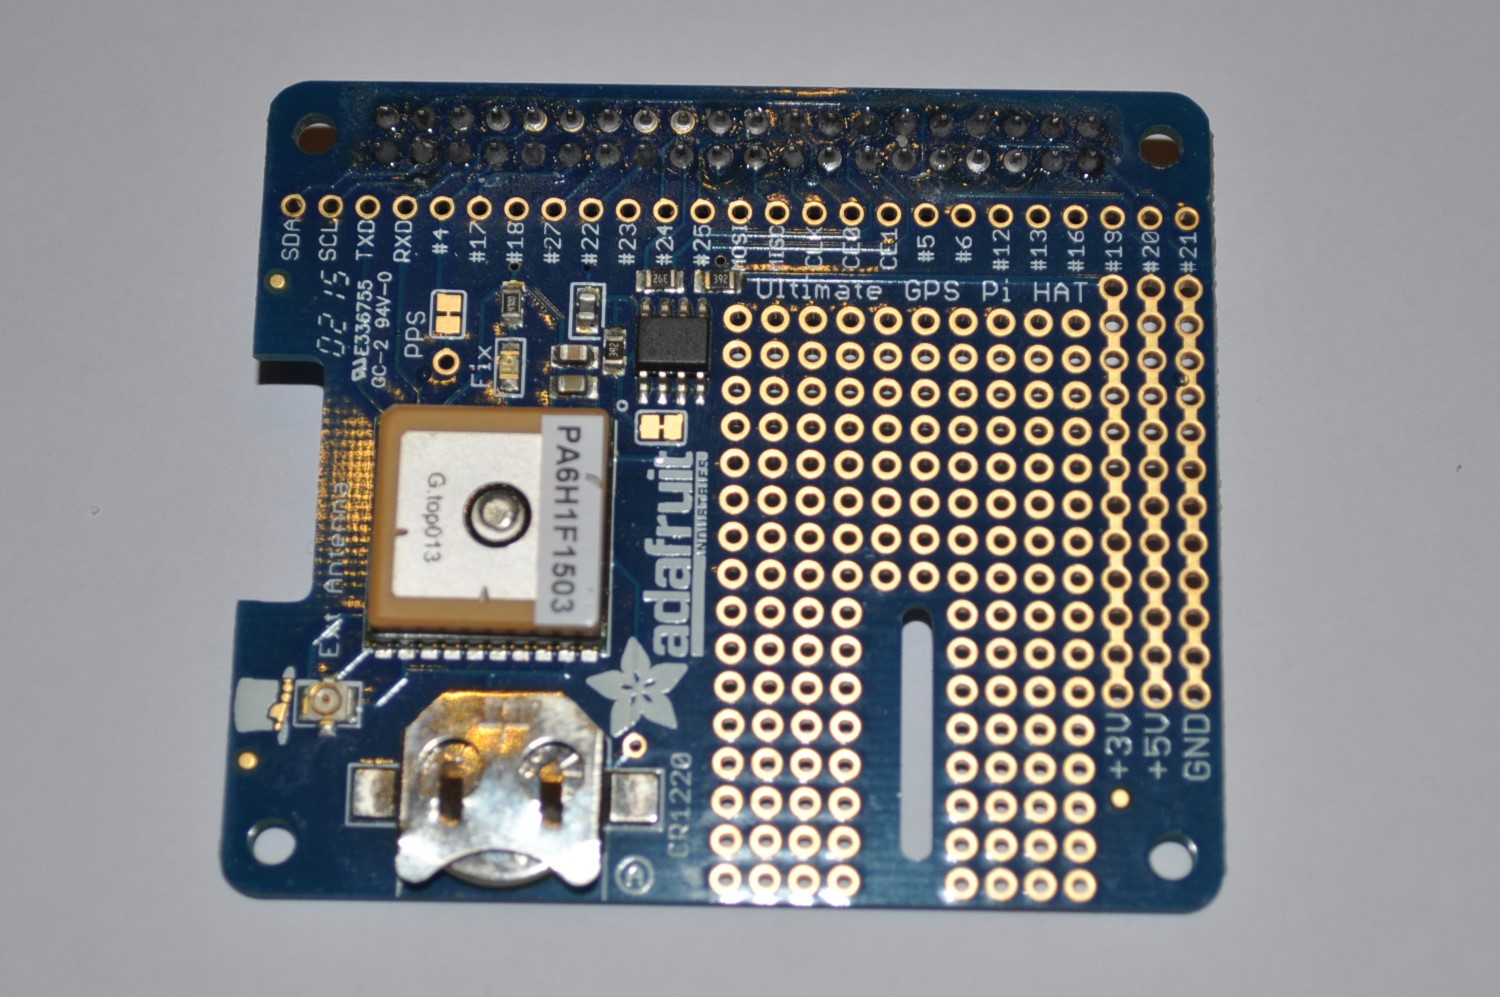
\includegraphics[width=0.48\textwidth]{bilder/DSC_0412}
\subsection{GPS Antenna}
We only used the internal \gls{gps} antenna for testing. Our problem was that it took really long to get a \gls{gps} signal every time we changed the location. With the external antenna it worked much quicker. In the final product an external antenna would not be necessary because the gps board remembers the last position and a position update is faster by orders of magnitude.\newline 
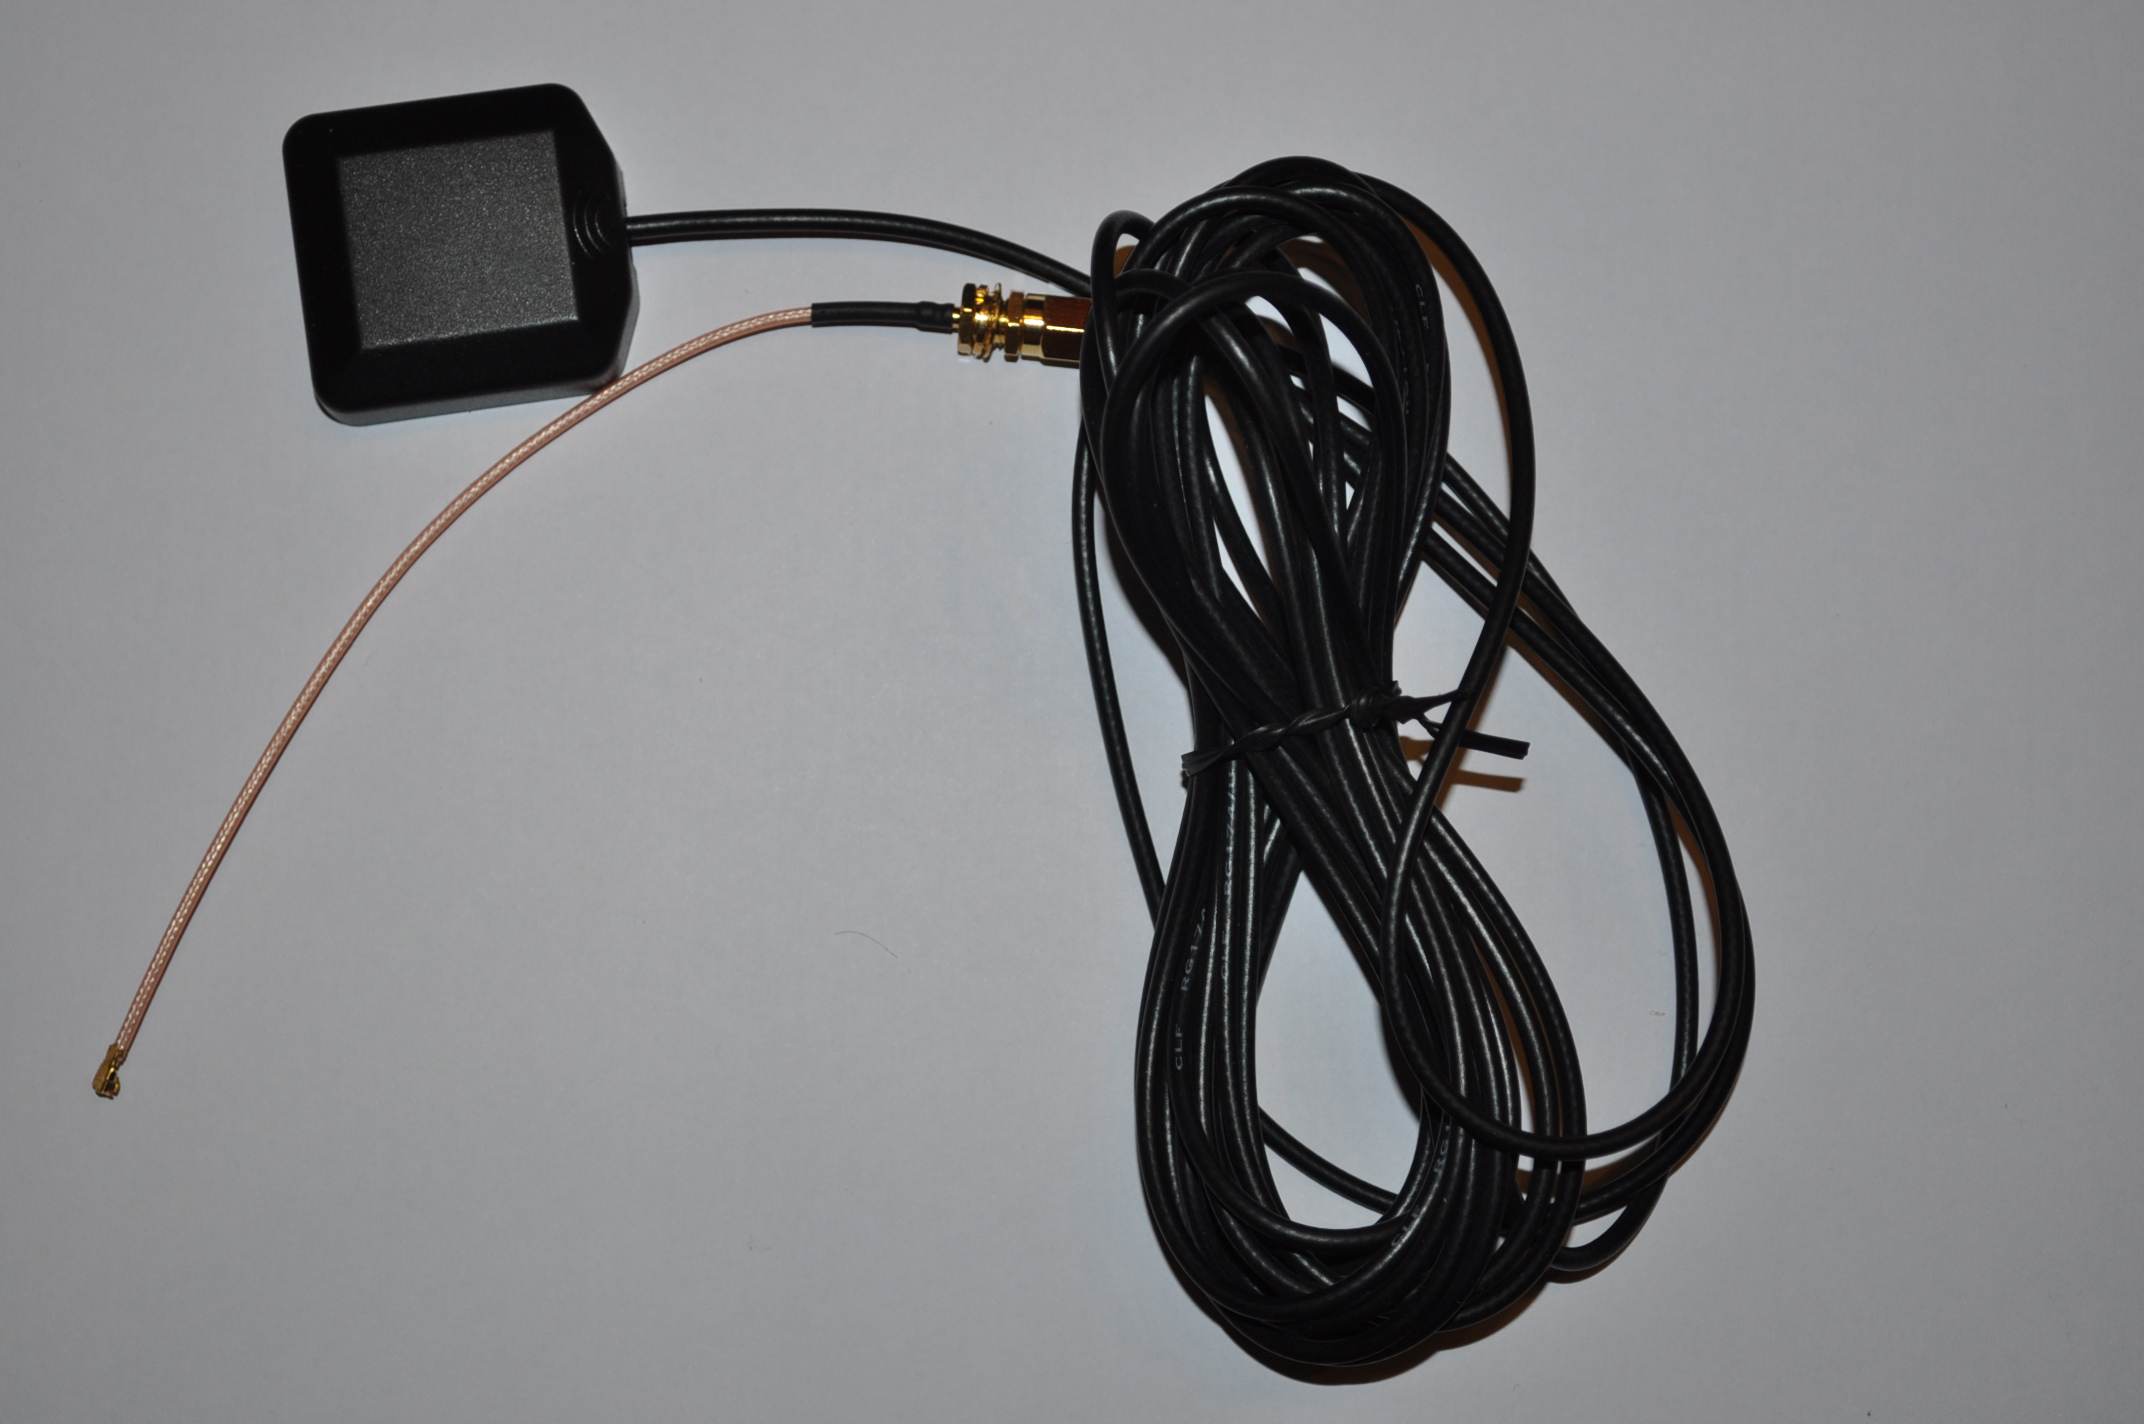
\includegraphics[width=0.48\textwidth]{bilder/DSC_0419}
\subsection{UMTS Stick}
The \gls{umts} stick is necessary for transmitting the data to the \gls{db}.\newline
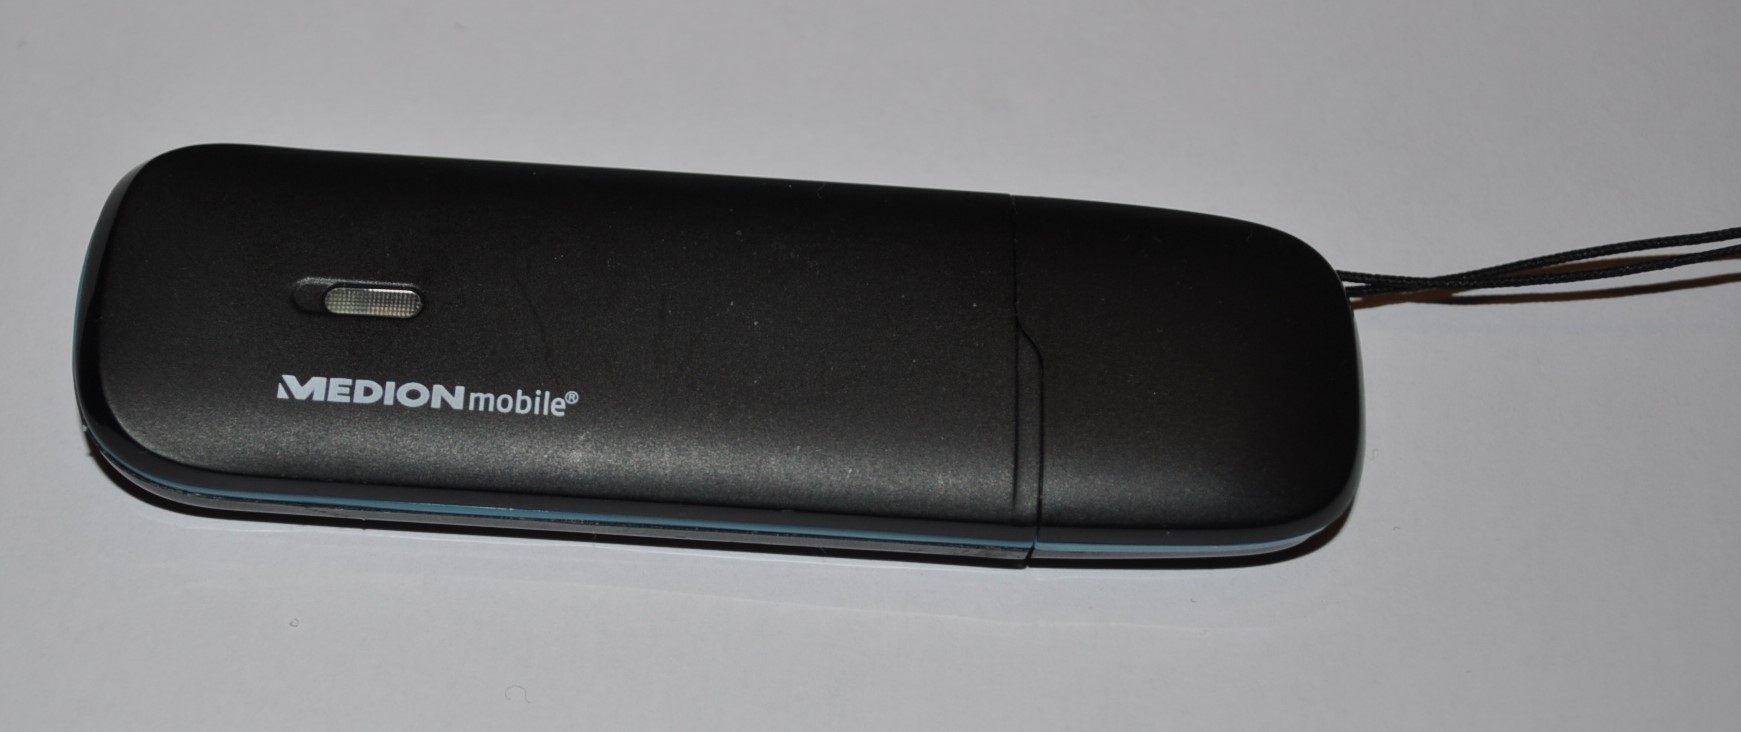
\includegraphics[width=0.48\textwidth]{bilder/DSC_0415}
\subsection{UPS}
If the engine of the car is switched off, the power supply of the \gls{rpi2} is interrupted. When the \gls{rpi2} gets power from the engine again, it has to do a system check and repair all files. Our final product will use an \gls{ups}. This \gls{ups} supplies our \gls{rpi2} with power even if the engine of the car is turned off. This eliminates the problem of data loss.\newline
%
\includegraphics[width=0.48\textwidth]{bilder/USV}
\newpage
\subsection{OS}
\subsubsection{Raspbian Wheezy}
When we started our diploma thesis the most common operation system on the \gls{rpi2} was and still is Raspbian Wheezy. At the beginning we downloaded the image and wrote the .img file on the microSD Card. You always have to connect the \gls{rpi2} to a screen to start Raspbian Wheezy. There you have to configure things like the keyboard layout. You can also do that later with the
\begin{minted}{python}
	sudo raspi-config
\end{minted}
command. After that you have to reboot the \gls{rpi2}.
Since we wanted to have a remote connection, we installed a \gls{tvnc} Server on the \gls{rpi2}. For this, we used the  
\begin{minted}{python}
	sudo apt-get install tightvncserver
\end{minted}
command.\newline
To connect the \gls{rpi2} via a \gls{tvnc} Client, we had to start the server with the 
\begin{minted}{python}
	tightvncserver
\end{minted}
command. Then the Server started on the Port 5901. For the connection establishment, we had to write the \gls{ip} address and the Port 5901 into the \gls{tvnc} Client. After that, we started to configure everything for the use of the \gls{gps} module.
\paragraph{GPS} \mbox{}\\
First we had to configure the communication between the \gls{rpi2} and the \gls{uart} pins on it. These \gls{uart} pins are \gls{gpio} 14 and 15.\newline
To stop the sending of the debug information, we had to edit the following file /boot/cmdline.txt with the 
\begin{minted}{python}
	sudo nano /boot/cmdline.txt
\end{minted}
command.\newline
There was one line within this text file and there the following text needed to be deleted
\begin{minted}{python}
	console=ttyAMA0,115200 kgdboc=ttyAMA0,115200
\end{minted}
Now it looked like this: 
\begin{minted}{python}
/dwc_otg.lpm_enable=0 console=tty1 root=/dev/mmcblk0p2 rootfstype=ext4 
elevator=deadline rootwait
\end{minted}
The \gls{rpi2} sends all terminal output over the external serial. To disable this behaviour, we had to edit the /etc/inittab file. We did this with the 
\begin{minted}{python}
	sudo nano /etc/inittab
\end{minted}
command.\newline
There we had to comment out the following line:
\begin{minted}{python}
#Spawn a getty on Raspberry Pi serial line
T0:23:respawn:/sbin/getty -L ttyAMA0 115200 vt100
\end{minted}
An interesting thing was, that this file did not exist on the Raspbian Jessie Lite image. There we had to change nothing.\newline
The next step was to ensure if the Raspbian was up-to-date. At the beginning we did that with the 
\begin{minted}{python}
	sudo apt-get update
\end{minted}
and the 
\begin{minted}{python}
	sudo apt-get dist-upgrade
\end{minted}
command. Then we had to restart the \gls{rpi2}. We waited, but the \gls{rpi2} did not boot. So to find out what's going on, we connected the \gls{rpi2} to a screen and looked at the output. It showed us something like that all CPU stopped and at the end there was a line that looked like this:
\begin{minted}{python}
	---[ end Kernel panic - not syncing: VFS: Unable to mount root 
	   fs on unknown-block(0,0)
\end{minted}
So we looked up for another option and found out that we should  use the 
\begin{minted}{python}
	sudo rpi-update
\end{minted}
command before rebooting. Searching for a fitting solution, we found many possibilities we had to try until we found the right one for our problem. So we started the whole process of ensuring if the Raspbian was up-to-date all over again. Actually we did this many times, for every possible solution we found.\newline
So after we used the 
\begin{minted}{python}
	sudo rpi-update
\end{minted} 
command and rebooted the \gls{rpi2}, we could finally continue.\newline
Now we had to download and configure the required packages. We had to use the pps-tools and the libcap-dev. We did this with the 
\begin{minted}{python}
	sudo apt-get install pps-tools
\end{minted}
and the 
\begin{minted}{python}
	sudo apt-get install libcap-dev
\end{minted}
commands. These commands are for displaying the \gls{gps} data on the command line.\newline
After that we also had to install the \gls{gpsd} with the following command:
\begin{minted}{python}
	sudo apt-get install gpsd gpsd-clients python-gps
\end{minted}
The \gls{gpsd} presents us the data over a small server.\newline
Before we could start the \gls{gpsd}, we had to kill all the running \gls{gpsd}'s. We did that with the 
\begin{minted}{python}
	sudo killall gpsd 
\end{minted}
command. Finally we could start it and use it with the 
\begin{minted}{python}
	sudo gpsd /dev/ttyAMA0 -F /var/run/gpsd.sock -G
\end{minted}
command.
\paragraph{GPS Data} \mbox{}\\
We had to test if the \gls{gps} was working. There are many command line interfaces presenting you the data so you can see something.\newline
There ist the 
\begin{minted}{python}
	sudo cgps -s
\end{minted}
command that shows following output: \newline
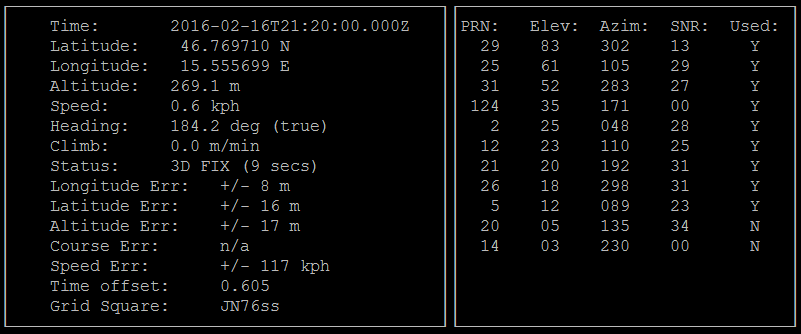
\includegraphics[scale=0.7]{bilder/scr1}
\newline
then the
\begin{minted}{python}
	sudo xgps
\end{minted}
command where you can see this:\newline
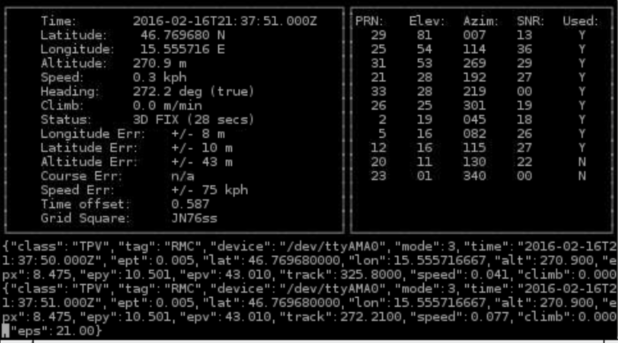
\includegraphics[scale=0.9]{bilder/scr2}
\newline
and at last the 
\begin{minted}{python}
	sudo gpsmon
\end{minted}
command to see following information: \newline
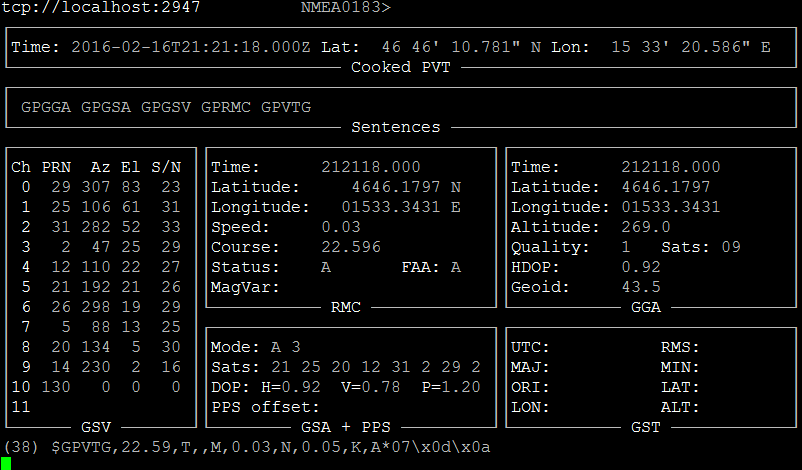
\includegraphics[scale=0.7]{bilder/scr3}
\newline
Then we wanted to save the \gls{gps} Data on the \gls{rpi2}. We did this with the 
\begin{minted}{python}
	gpspipe -r | grep '^\$G' | tee test.nmea 
\end{minted}
command.
But since we could not use the \gls{nmea} format, we had to transform it into something like \gls{gpx} or \gls{kml}. For that we used the GPSBabel command line program. GPSBabel converts \gls{gps} data into other formats and saves it into a file. But firstly we had to install GPSBabel with the 
\begin{minted}{python}
	sudo apt-get install gpsbabel 
\end{minted}
command. We converted it into both, \gls{kml} and \gls{gpx} and for that we had to use the two following commands.
To get a KML file, we used:
\begin{minted}{python}
	gpsbabel -i nmea -f test.nmea -o kml -F test.kml
\end{minted}
To get a GPX file, we used:
\begin{minted}{python}
	gpsbabel -i nmea -f test3.nmea -o gpx -F test3.gpx
\end{minted}
\paragraph{Software development} \mbox{}\\
After we applied these commands, we started programming. We all know the programming language JAVA the best, so we decided to use it for our software.  

We looked for an \gls{api} for JAVA and found one and a small test program with it. \newline
But we needed JAVA on the \gls{rpi2} to run a JAVA program. We wanted to use JAVA 8, but there was no real JAVA 8 \gls{jdk} for the \gls{rpi2}, so we had to use JAVA 7. We installed it with the following command:
\begin{minted}{python}
	sudo apt-get install oracle-java7-jdk
\end{minted}
You can read later everything about the program.

\paragraph{Auto boot} \mbox{}\\
While developing we started our program mostly from our own notebooks, but in the final product we wanted it to start automatically after booting for further use. For the final product everything has to start after booting anyway. So we edited the /etc/rc.local file with the 
\begin{minted}{python}
	sudo nano /etc/rc.local
\end{minted} 
command. At the last position we added the line
\begin{minted}{python}
	/home/pi/autostart.sh 
\end{minted} 
This means, that the autostart.sh, that was created by us, will be called upon when the \gls{rpi2} starts. Then we created the autostart.sh with the 
\begin{minted}{python}
	nano autostart.sh
\end{minted}
command. In in this file we wrote:
\begin{minted}{python}
	#!/bin/sh

	sudo killall gpsd
	sudo gpsd /dev/ttyAMA0 -F /var/run/gpsd.sock -G
\end{minted}
To make the script executable we had to use the following command:
\begin{minted}{python}
	chmod +x autostart.sh
\end{minted}
\paragraph{Problems} \mbox{}\\
Here we are going to explain some problems which appeared and did not mention before.\newline
Since we had a \gls{wlan} stick, we wanted the \gls{rpi2} to be connected with a router. We found out, that the /etc/network/interfaces file must be edited. This was done with the
\begin{minted}{python}
	sudo nano /etc/network/interfaces 
\end{minted}
command.\newline
At the beginning it looked like this:
\begin{minted}{python}
	auto lo
	iface lo inet loopback

	auto eth0
	allow-hotplug eth0
	iface eth0 inet dhcp

	auto wlan0
	allow-hotplug wlan0
	iface wlan0 inet manual
	wpa-conf /etc/wpa_supplicant/wpa_supplicant.conf

	auto wlan1
	allow-hotplug wlan1
	iface wlan1 inet manual
	wpa-conf /etc/wpa_supplicant/wpa_supplicant.conf
\end{minted}
Then we changed the \gls{wlan} interface.
\begin{minted}{python}
	auto wlan0
	allow-hotplug wlan0
	iface wlan0 inet dhcp
	wpa-ssid "linksys"
	wpa-psk "raspberry"
\end{minted}
This worked out quite well, but if the \gls{rpi2} started and there was no \gls{wlan}, the \gls{rpi2} did not accept \gls{lan} too.
\newpage
\subsubsection{RASPBIAN JESSIE LITE}
Jessie Lite is a command line \gls{os}. Our final product will run on this \gls{os}, because it's starting much faster than Raspbian Wheezy. Additionally, Raspbian Wheezy is no longer updated since 2015 and isn't able to be downloaded from the official site since February 2016.
\paragraph{Getting started} \mbox{}\\
At the beginning we downloaded the Raspbian Jessie Lite image and wrote the .img file on the microSD Card. There was the first problem. The old Raspbian Wheezy image set the partition size to the maximum while booting. With Jessie Lite we had to do that on our own. 

The next problem was that the ethernet interfaces \gls{ip} was set to manual. Wheezy had set it to auto. So, if we want to have internet access from the beginning, we had to edit the interface file (/etc/network/interfaces) before booting the \gls{rpi2}. Since we did it after the boot, too, we are going to describe how to do that later and there you can also see what we changed in this file.

The next step was to edit the boot file(/boot/cmdline.txt). When this was carried out, the \gls{gpsd} received data from the pins. We changed the same at the ethernet interface later. In this file was no difference when we did it. 
\newline \newline
Here we had to remove 
\begin{minted}{python}
	console=ttyAMA0,115200
\end{minted}
Then it looked like this: 
\begin{quote}
\begin{verbatim}
	dwc_otg.lpm_enable=0 console=tty1 root=/dev/mmcblk0p2 
	rootfstype=ext4 elevator=$
\end{verbatim}
\end{quote}
After these applied changes, we inserted the microSD Card into the \gls{rpi2} and plugged it in.
\paragraph{GPS Configuration} \mbox{}\\
If we would not configure the ethernet interfaces \gls{ip} to manual, we have to connect the \gls{rpi2} to a screen. Then we edited the interface file(/etc/network/interfaces). This can be done with the 
\begin{minted}{python}
	sudo nano /etc/network/interfaces
\end{minted}
command. \newline
In this file there is a line iface eth0 inet manual and instead of this line we had to write:
\begin{minted}{python}
	auto eth0
	allow-hotplug eth0
	iface eth0 inet auto
\end{minted}
Then we rebooted the \gls{rpi2} and accessed it over the \gls{lan}. \newline
If we had not done it before, we would have to edit the boot file(/boot/cmdline.txt) with the following command:
\begin{minted}{python}
	sudo nano /boot/cmdline.txt
\end{minted}
There we removed console=ttyAMA0,115200 from the first line.\newline
After that we checked if everything was up to date with the following two commands:
\begin{minted}{python}
	sudo apt-get update
	sudo apt-get dist-upgrade
\end{minted}
Next we had to install different programs to get the \gls{gps} data.\newline
First we installed pps tools with the 
\begin{minted}{python}
	sudo apt-get install pps-tools
\end{minted}
command, the libcap dev with the 
\begin{minted}{python}
	sudo apt-get install libcap-dev
\end{minted}
command, and then the \gls{gpsd} with the 
\begin{minted}{python}
	sudo apt-get install gpsd gpsd-clients python-gps
\end{minted}
command.\newline
Since our program is written in JAVA, we also had to install JAVA with the 
\begin{minted}{python}
	sudo apt-get install oracle-java7-jdk
\end{minted}
command.\newline
Some other changes we had to apply on the Jessie Lite image, were editing the \gls{gpsd} file. We edited it with this command:
\begin{minted}{python}
	sudo nano /etc/default/gpsd
\end{minted}
Below you can see the whole file with our changes. 
\begin{minted}{python}
	# Default settings for the gpsd init script and the 
	hotplug wrapper.

	# Start the gpsd daemon automatically at boot time
	START_DAEMON="true"

	# Use USB hotplugging to add new USB devices 
	automatically to the daemon
	USBAUTO="false"

	# Devices gpsd should collect to at boot time.
	# They need to be read/writeable, either by user gpsd 
	or the group dialout.
	DEVICES="/dev/ttyAMA0"

	# Other options you want to pass to gpsd
	GPSD_OPTIONS=""

	# Additionally:
	GPSD_SOCKET="/var/run/gpsd.sock"
\end{minted}
\paragraph{Copy program on RPi2} \mbox{}\\
Now we had to copy the program on the \gls{rpi2}. We wanted to do that via \gls{usb} stick. But there was the next problem. With the old Wheezy image we just connected the \gls{usb} stick. With the Jessie Lite image we had to mount the stick. We created a new folder called usb in the /mnt/ directory.
\begin{minted}{python}
	sudo mkdir usb
\end{minted}
Then we had to mount the \gls{usb} stick. We did this with the
\begin{minted}{python}
	sudo mount /dev/sda1 /mnt/usb/ -o uid=1000
\end{minted}
command. If we wanted to unplug the \gls{usb} stick we had to use the 
\begin{minted}{python}
	sudo umount /mnt/usb
\end{minted}
command.\newline
Then had to copy the .tar.gz file to /opt with the \begin{minted}{python}
	sudo cp gps.tar.gz /opt
\end{minted}
command. To extract it, we used the 
\begin{minted}{python}
	sudo tar xzvf gps.tar.gz
\end{minted}
command.\newline

\paragraph{Autostart(as Daemon)} \mbox{}\\
We created a gps\_rest.service script and put it into a folder near our program called systemd. Our script looks like this:
\begin{minted}{python}
	[Unit]
	Description=GPS Rest Daemon PaClLaHell
	[Service]
	ExecStart=/sbin/start-stop-daemon --start --quiet --make-pidfile 
	--pidfile /var/run/gps_rest.pid --background --user pi --chuid pi 
	--chdir /opt/gps --exec /usr/bin/java -- -jar GPS_REST.jar
	ExecStop=/sbin/start-stop-daemon --stop --quiet --pidfile 
	/var/run/gps_rest.pid --user pi --chuid pi --exec /usr/bin/java
	Type=forking
	[Install]
	WantedBy=multi-user.target
\end{minted}
%versteh den nächsten satz nicht
Then in /etc/systemd/system/multi-user.target.wants we create a like too the gps\_rest.service (\textit{sudo ln -s /opt/gps/systemd/gps\_rest.service}).
After that we rebooted the \gls{rpi2} and started the GPS\_REST.jar as a daemon.
To start and stop the daemon, we used following commands:
\begin{minted}{python}
	sudo systemctl start gps_rest.service
	sudo systemctl stop gps_rest.service
\end{minted}
And to get information about the daemon we used this command:
\begin{minted}{python}
	sudo systemctl status gps_rest.service
\end{minted}
\paragraph{UMTS Stick} \mbox{}\\
Since the \gls{umts} stick is not the newest, it was not that easy to make it working with the \gls{rpi2}.
\subparagraph{Configure the USB config} \mbox{}\\
At first we had to configure the \gls{rpi2} so it would accept the stick as a modem.\newline
We created a file in /opt/gps/udev and there we had to name this file 70-usb-modeswitch.rules. In this file we had to add this line:
\begin{minted}{python}
	ACTION=="add", SUBSYSTEM=="usb", 
	ATTRS{idVendor}=="0e8d", 
	ATTRS{idProduct}=="0002", 
	RUN+="/usr/sbin/usb_modeswitch -v 0e8d -p 0002 -M 
	'555342431234567800000000000006f0010300000000000000000000000000'"
\end{minted}
Then we had to create a link to the right position, that was /opt/gps/udev/rules/. This has been done with the 
\begin{minted}{python}
	sudo ln -s /opt/gps/udev/rules/70-usb-modeswitch.rules
\end{minted}
command.\newline
After that the following command showed us if the ID from the stick was right.
\begin{minted}{python}
	lsusb
\end{minted}
\subparagraph{Configuration of the provider}\mbox{}\\
To make configurations, we had to change to the super user state, with the 
\begin{minted}{python}
	sudo su
\end{minted}
command.\newline
After that we had to create two files with information for ppp. \newline
We created the first file called hot\_internet in /etc/chatscripts/. \newline
In this file we had to put these lines:
\begin{minted}{python}
	TIMEOUT 10
	ABORT 'BUSY'
	ABORT 'NO ANSWER'
	ABORT 'ERROR'
	ABORT 'NO CARRIER'
 
	'' 'ATZ'
	'OK' 'ATE1'
	'OK' 'AT+CGDCONT=1,"IP","webaut","0.0.0.0",0,0'
	'OK' 'ATDT*99#'
	'CONNECT' '\c'
\end{minted}
The next file was also called hot\_internet and created in /etc/ppp/peers/.\newline
This file looked like this:
\begin{minted}{python}
	hide-password
	noauth
	connect "/usr/sbin/chat -v -f /etc/chatscripts/hot_internet"
	debug
	/dev/ttyUSB0
	115200
	defaultroute
	replacedefaultroute
	noipdefault
	usepeerdns
	crtscts
	lock
	local
	 
	# Redial and interval
	persist
	holdoff 5
	 
	# No compression
	novj
	novjccomp
	nopcomp
	nodeflate
		 
	# PAP authentication
	 
	# LCP echo messages settings
	lcp-echo-failure 4
	lcp-echo-interval 65535
\end{minted}
After that we could start it with 
\begin{minted}{python}
	pon hot_internet
\end{minted}
and stop it with 
\begin{minted}{python}
	poff hot_internet
\end{minted}
\subparagraph{Auto boot PPP}\mbox{}\\
When pon/poff worked, we had to configure the /etc/network/interfaces and here we had to add the ppp interface as you can see in the following code lines:
\begin{minted}{python}
	# interfaces(5) file used by ifup(8) and ifdown(8)
	 
	# Please note that this file is written to be used with dhcpcd
	# For static IP, consult /etc/dhcpcd.conf and 'man dhcpcd.conf'
 
	# Include files from /etc/network/interfaces.d:
	source-directory /etc/network/interfaces.d
	 
	auto lo
	iface lo inet loopback
	 
	auto eth0
	iface eth0 inet dhcp
	 
	allow-hotplug ppp0
	auto ppp0
	iface ppp0 inet ppp
	provider hot_internet
	 
	allow-hotplug wlan0
	iface wlan0 inet manualrp
	    wpa-conf /etc/wpa_supplicant/wpa_supplicant.conf
	 
	allow-hotplug wlan1
	iface wlan1 inet manual
	    wpa-conf /etc/wpa_supplicant/wpa_supplicant.conf
\end{minted}
\textbf{References:} \cite{gpsd}, \cite{USBModeSwitch}, \cite{GSMmobile}, \cite{USBModemStickMedion}, \cite{PPPunderUbuntu}, \cite{USBSurfstick}, \cite{Reboot}, \cite{DaemonizeJavaApplications}, \cite{raspberrypi}, \cite{Tastaturlayout}, \cite{TightVNCServer}, \cite{RaspberryPiGPS}, \cite{gpsbable}, \cite{autostartScript}, \cite{wlan}
\clearpageauthor
\newpage
\section{Software Description}
\pageauthor{Laura Rössl}
The software of our \gls{rpi2} consists of two threads and a blocking FileObjectQueue. We get the \gls{gps} data from the \gls{api} and upload it via \gls{rest} in the \gls{db}. 
\subsection{Functions}
First of all a logging property file and a gps property file are loaded. The logging property file contains logging information like the saving location and the maximum number of logging files. The gps property file contains the raspberry id, the server \gls{url} and the gps module \gls{ip}.
\subsection{GPS API}
The \gls{api} (Gpsd4java) manages the connection with the \gls{gps} daemon, that covers receiving data, parsing this information into an useful format and supplying it to the “API Thread”. The \gls{gps} data we use consists of the timestamp, coordinateX, coordinateXError, coordinateY, coordinateYError, acceleration, altitude and altitudeError.
\subsection{Tape API}
We implemented this \gls{api}, because of the problem with saving data into an offline file. This \gls{api} provides us a FileObjectQueue where we can put and remove our points and this FileObjectQueue is automatically saved in a file. 
\subsection{Save Thread}
The Save thread reads point data from the FileObjectQueue and sends the data to the \gls{rest} server. When the tracks are written in the database, the Save Thread removes these points from the FileObjectQueue.
\subsection{API Thread}
When the GPS API measures \gls{gps} data, the API Thread gets it from the \gls{api}. The API Thread adds the information about the track and loads it into the FileObjectQueue.
\begin{center}
\includegraphics[width=1\textwidth]{bilder/SoftwareDiagram1}
\end{center} 
\subsection{PHP (REST)}
This part of our software is responsible for the upload into the database. The \gls{rest} server gets the data formatted as \gls{json}.\\
\paragraph{lines of code}\mbox{}\\
Paul Zwölfer: 119 lines
\begin{center}
\includegraphics[width=1\textwidth]{bilder/SoftwareDiagram2}
\end{center} 
\clearpageauthor
\section{Code Structure}
\pageauthor{Paul Zwölfer}
\subsection{Classes}
\subsubsection{GPS.java}
\paragraph{Constructor}\mbox{}\\
In the GPS.java class, the gpsModuleAddress variable is initialized and gets its value from the GPSConfiguration.java class.
\paragraph{startGpsdClient}\mbox{}\\
In the startGpsdClient method, the GPS API is initialized and the validate method from the BL.java class is called every time we get data from the GPS API.
\paragraph{lines of code}\mbox{}\\
Laura Rössl: 50 lines \\
Paul Zwölfer: 29 lines
\subsubsection{BL.java}
\paragraph{Constructor}\mbox{}\\
In this class the FileObjectQueue is created and initialized by the save.jPoint file and the GsonConverter.java class. 
Then a new track is created and at last the SaveDataThread object is initialized and started.
\paragraph{Validate}\mbox{}\\
Checks if the data from the GPS API is a number. If not it will be set to 0 except the latitude and the longitude. If they are \gls{nan} it will do nothing. 
Then it adds the data from the GPS API to the FileObjectQueue.
\paragraph{ProcessData}\mbox{}\\
This method peeks max 50 and min 15 points from the FileObjectQueue and puts them into a JContainer. Then it sends these points to the DataManager.java class to upload them via the uploadContainer method.
\paragraph{lines of code}\mbox{}\\
Paul Zwölfer: 184 lines
\subsubsection{SaveDataThread.java}
This is an intern Class in the \gls{bl} class that extends Thread.
\paragraph{Run}\mbox{}\\
This override method calls the ProcessData method and then waits 1 second.
\subsubsection{Data Manager.java}
\paragraph{Constructor}\mbox{}\\
Gets the server \gls{url} and puts it on the urlString variable.
\paragraph{UploadContainer}\mbox{}\\
Uploads the JContainer it got to the Server via \gls{rest}.
\paragraph{lines of code}\mbox{}\\
Paul Zwölfer: 73 lines
\subsubsection{JContainer.java}
This is a beans class that contains attributes, getter and setter methods for the respective attribute and a toString method of the JContainer.
\paragraph{lines of code}\mbox{}\\
Claudio Knapp: 25 lines\\
Paul Zwölfer: 62 lines
\subsubsection{JPoint.java}
This is a beans class that contains attributes, getter and setter methods for the respective attribute and a toString method of the JPoint.
\paragraph{lines of code}\mbox{}\\
Claudio Knapp: 55 lines \\
Paul Zwölfer: 158 lines
\subsubsection{GPSConfiguration.java}
At the beginning this class loads the logging properties.
\paragraph{InitConfiguration}\mbox{}\\
Reads the properties for the program from a file and sets these values on the specified variables. If a value is not in the file, it sets a default value. And at the end it closes the file.
\paragraph{lines of code}\mbox{}\\
Paul Zwölfer: 95 lines
\subsubsection{GsonConverter.java}
This class is a converter class that has implemented a FileObjectQueue Converter. In the method, the bytes from the file are converted, so that they can be saved on the FileObjectQueue. In the toStream method, it is the other way round, so the FileObjectQueue is saved on a file.
\paragraph{lines of code}\mbox{}\\
Paul Zwölfer: 53 lines
\subsection{Class Diagram}
\begin{center}
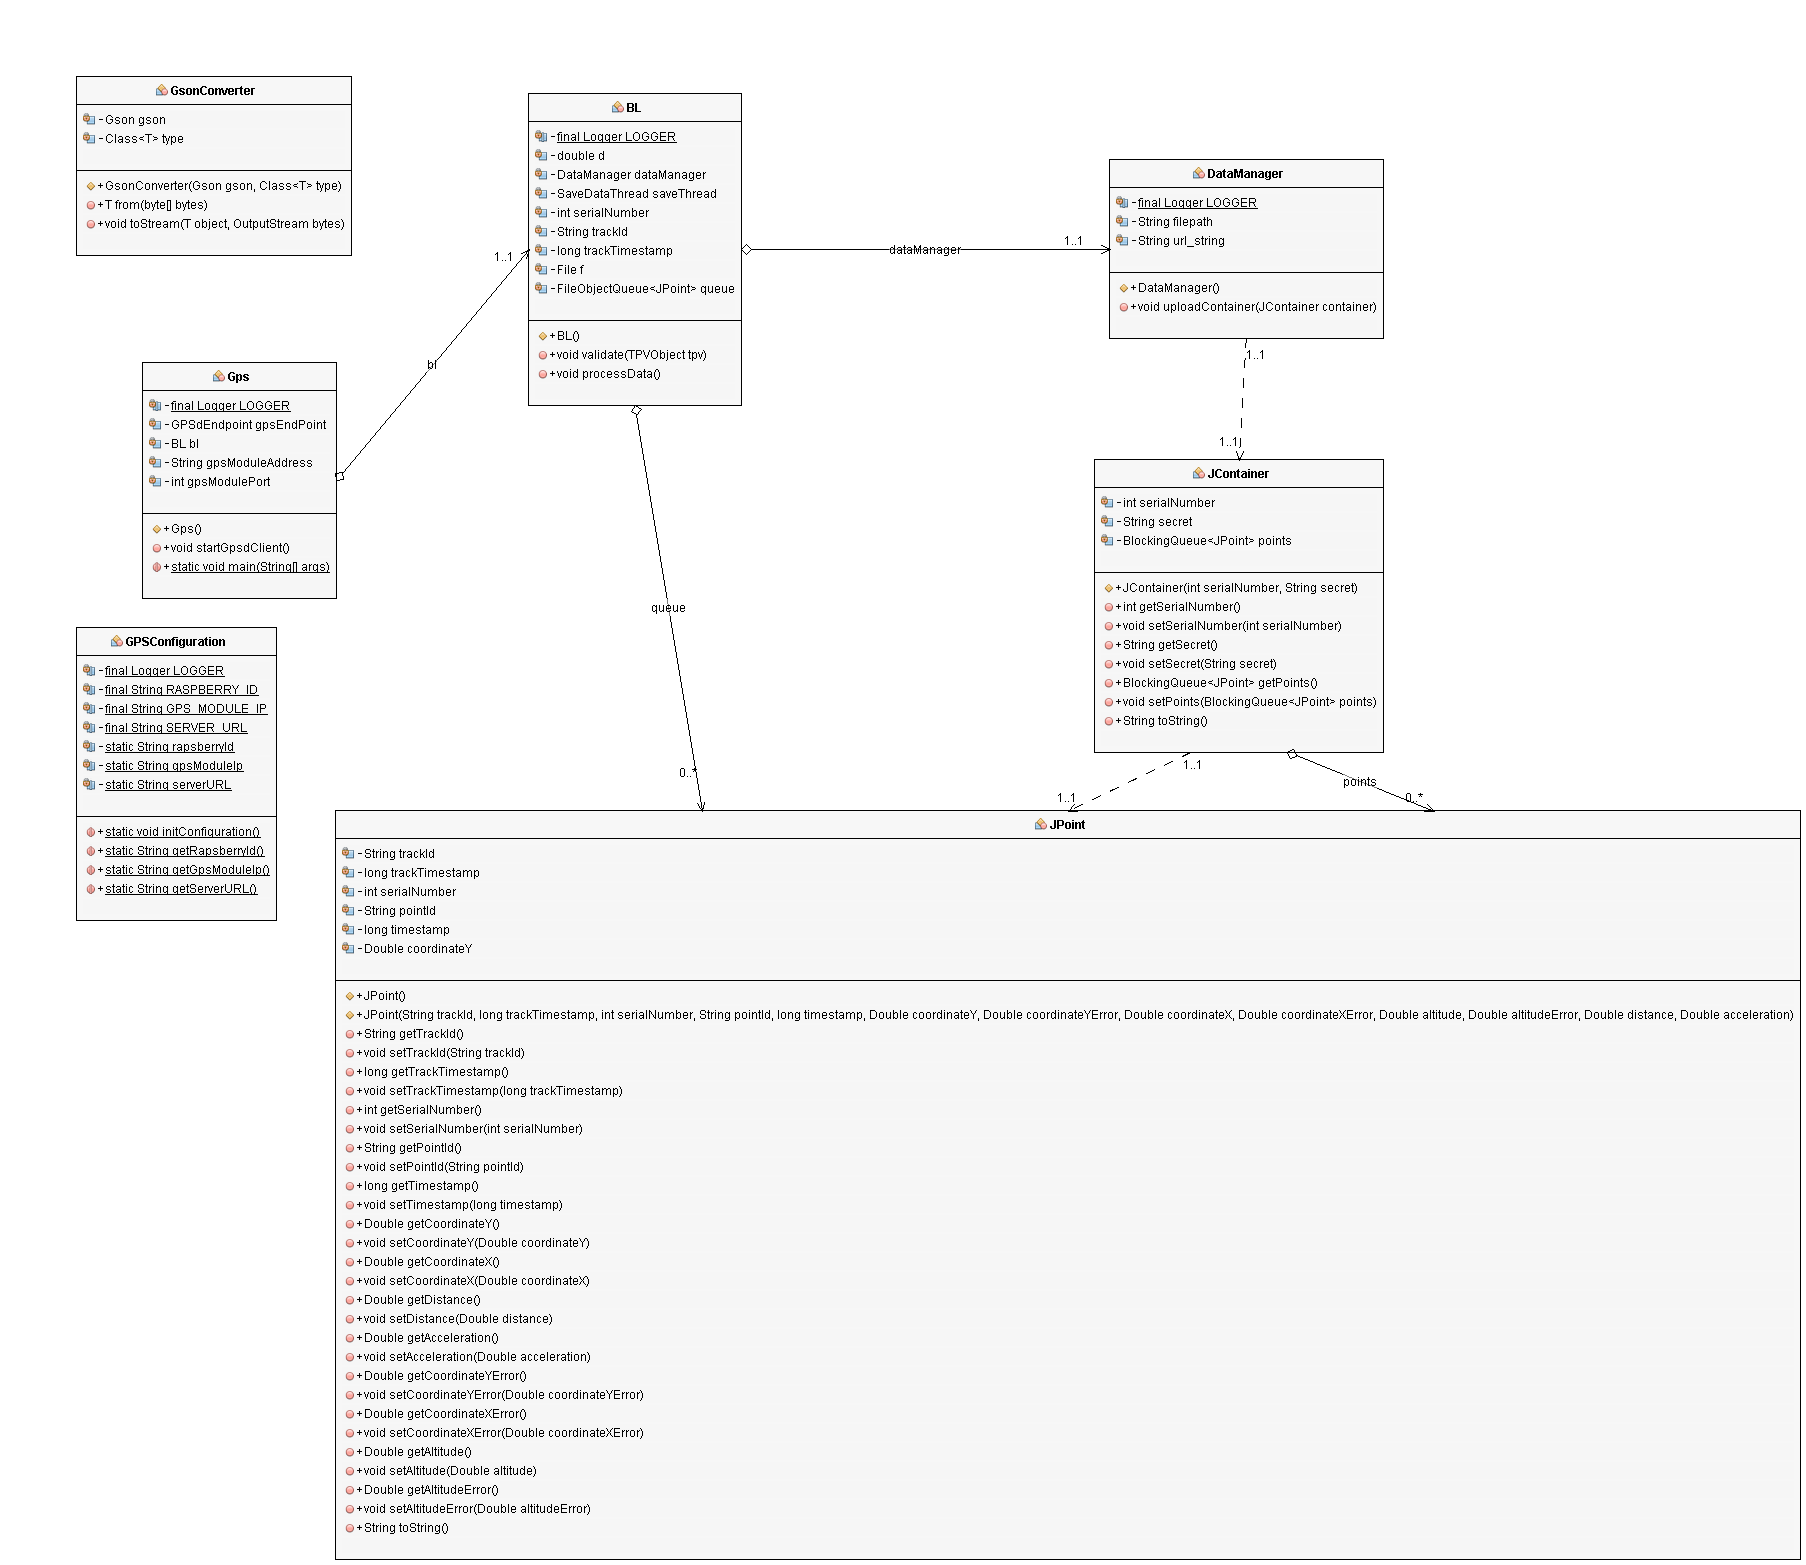
\includegraphics[width=1\textwidth]{bilder/GPS_REST_UML_Diagram}
\end{center}
\clearpageauthor
\section{Problems}
\pageauthor{Claudio Knapp}
\subsection{Uploading into Database}
When we started with this project, we uploaded tracked data directly into the database over a standard java database connection. Beside working on this project, we learned the technology hibernate in school so we reconstructed our program and used hibernate. Later our employer told us, that we should use \gls{rest} to upload data for a higher security level and fewer connections to the database and therefore less overhead. Another reason why we had to use this web service technology is that it's not possible to directly access the \gls{db} from outside. We wrote the \gls{rest} \gls{php} script on our own. 
\subsection{Offline Saving}
When the engine stopped while saving data offline, we had a loss of points, because the whole save file we used was overwritten. So we created a copy of this file, removed the data that was already in the database and deleted the original file. Then we renamed the copy to the original file name. Nevertheless, there was still a problem. On the one hand, it was possible that no data was lost, but on the other hand everything could be lost if the power was cut off between deleting the original file and renaming the copy. This is the reason why we use Tape API now. 
\section{Functional Testing}
To ensure functionality of the hardware prototype and the software, we had to do several tests. They reach from logical problems to practical testing on the road.
\subsection{Database Connection Error}
While developing our software, the error handling when loosing database connection was a very important issue. We had to think about different solutions for different code structure because we changed the database connection type several times. 
\newline \newline
We decided on the connection type called \gls{rest}. When using a technology that relies heavily on a working internet connection, there had to be a backup plan if exactly this connection is not working anymore.
\newline \newline
When does an connection error occur:
\begin{itemize}
\item internet not working
\item database not working/running
\end{itemize}
We decided on saving points, that cannot be uploaded, into a \gls{json} (save.jPoint). This solution proved to be the most fitting idea we thought of. It perfectly handled the described problems, reliably managed points and the saving mechanism worked phenomenal.
\newline \newline
The same concept is used when the database is offline or not working properly. 
\subsection{Inaccuracy of the GPS Coordinates}
After the first tests, where we tried to get \gls{gps} signal, we noticed a slight inaccuracy of the signal. This inaccuracy gets influenced by several factors. Therefore we had to find out how precise our \gls{gps} coordinates are and how much of an imprecision (part of the \gls{gps} data we get from our module) there is. 
\newline \newline
We evaluated driven tracks and measured how much distance there is between the actual location and the \gls{gps} coordinates received. This difference was about 5 metres, so no problem at all. 
\newline \newline
Due to the fact that we receive how much of an inaccuracy there is in the \gls{gps} data, our partner company can easily extract this information and compensate it in the visualization process. To do that even better, we also saved the deviation and the altitude.

\begin{center}
%grafiken der gefahrenen strecken --> claudio
%\includegraphics[width=1\textwidth]{}
\end{center}

\subsection{No GPS Signal}
When handling the \gls{gps} inaccuracy, we had to take into account that there could be no signal at all. Therefore we had to decide on a solution when receiving this data and how to handle and save it.
\newline \newline
We tried different solutions, but finally decided on not saving them. It is the most efficient way concerning storage, both offline and online.
\newline \newline
Meaning of not saving data when having no signal:
\begin{itemize}
\item when there is no \gls{gps} signal, there is often also no internet connection
\item this leads to offline stored “null” points
	\begin{itemize}
	\item not saving these null points is the best solution
	\end{itemize}		
\item data extraction for our partner company when displaying the data on maps will be easier
\end{itemize}
\textbf{References:}  \cite{Git}, \cite{Gpsd4java}
\clearpageauthor
\newpage
\section{Future Work and Ideas}
\pageauthor{Claudio Knapp}
Due to our limitation in time, we cannot infinitely improve our program. Therefore we sum up our future ideas on what could be implemented or improved. Of course, we only write about the things that came up to our minds, and therefore this is just a small list.
\paragraph{Security between RPi2 and REST service}\mbox{}\\
As we found out during the implementation process, \gls{rest} supports an encryption process. After consulting the partner company, we decided on not using the encryption on the prototype.
\paragraph{Access via SSH over UMTS}\mbox{}\\
It should be possible to access the \gls{rpi2} over the internet via \gls{ssh} for remote maintenance.
\paragraph{Critical error reporting}\mbox{}\\
If a severe problem happens, \gls{rpi2} should be able to report that problem so that it can be fixed.
\paragraph{Mobile Application/Webform}\mbox{}\\
Using the wireframing of the webform and mobile devices, it is possible to create an access interface that can be accessed via a web browser or a mobile application.
\paragraph{Putting the GPS Points on the street}\mbox{}\\
As shown in the Functional Testing part, the \gls{gps} data is rather inaccurate. Therefore our partner company has to interpolate and/or use the inaccuracy we add to the uploaded data. This task was not possible not accomplish in the given time, but could be implemented afterwards.

Compensating the inaccuracy will help to get an exact distance measurement and provide a better user experience.
\paragraph{Optimize Http overhead}\mbox{}\\
If there are many points on the \gls{rpi2}  and the connection is established, the connection should only be closed after sending all the Points.
\clearpageauthor